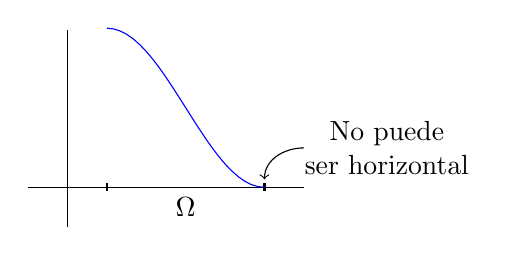
\begin{tikzpicture}

\draw (-0.5, 0) -- (3, 0);
\draw (0, -0.5) -- (0, 2);

\draw[thick] (0.5, -0.05) -- (0.5, 0.05);
\draw[thick] (2.5, -0.05) -- (2.5, 0.05);

\draw[blue, samples=25, domain=0:pi] plot ({\x / pi * 2 + 0.5} , { (1+cos(\x r)) * 1.01 });
\draw (3, 0.5) edge[out=180,in=90,->] (2.5, 0.1) node[xshift=30pt, align=center]{No puede\\ser horizontal};

\node at (1.5, -0.25) {$\Omega$};

\end{tikzpicture}